In this appendix we describe the Casanova extension that allows supporting networked games. This appendix starts by identifying the problem of creating networked games, it then describes how games solve the problem, and finally it outlines our solution.

Note that in the following we assume a host-client architecture where an authoritative host maintains the most updated version of the game world, and clients rely on the host to send them the updated game world at regular intervals.


\section{Networking and games}
Networking in games is a difficult problem to solve \cite{APPENDIX_B_NETWORKING_DIFFICULTIES}. Multiplayer requires the ability to synchronize the players game states so that they all see the same game in action, within the following set of requirements: \textit{(i)} synchronization has to happen in real-time; \textit{(ii)} communication cannot be blocking and synchronous or the player will have the feeling that the game has frozen during blocking calls, for example to send local input to the game host; \textit{(iii)} reliable channels cannot be employed because they use too much bandwidth; \textit{(iv)} old information often needs to be discarded, because entities update so quickly that their status is transmitted multiple times.

We define the problem of networking in terms of a known problem called \textit{eventual consistency} \cite{APPENDIX_B_EVENTUAL_CONSISTENCY}. We are not interested in creating a game where at every instant of the game all distributed players see exactly the same thing. 
% todo: rewrite block
Rather, we wish for the game instances to all work correctly, with minimal errors, but also with apparently immediate responses and smooth working. From this point of view then, it is not crucial that synchronization is perfect, and local predictions are allowed and even desirable. We must leave room for imprecise synchronization with periodic corrections, instead of designing and inflexible and low-performance mechanism which ensures perfect synchronization.

Networking code also presents further problems. A general-purpose solution to creating multiplayer games has not, as of now, been presented. We argue this to be due to the fact that such a solution is heavily dependent on how the game world is actually represented, its layout, and its semantics. Without some degree of understanding of the game world structure it is very hard to create a networked game automatically. The best efforts in this direction are not related to games, and use reflection in order to wholly and reliably transfer a data structure across a network \cite{APPENDIX_B_SERIALIZATION}. These solutions are not feasible for games since they are low-performance, they use too much bandwidth in ensuring that all the data comes through, and they do not account for the fact that the same datum will be transmitted again very soon, or that it was transmitted some time before and thus parts of the previous transmission should be reused.

Our experience also shows that networking code also pollutes the game sources, hindering their readability. The game logic and rendering, which maintain useful properties about our entities, often need to be accompanied by data about the networking protocol. Networking related data will often contain at least: \textit{(i)} a unique ID to identify the entity across the various distributed instances of the game; \textit{(ii)} the amount of time since the last transfer of a value in order to decide when to send it in full again; \textit{(iii)} whether or not an entity has been received by the last transmission for the occasional reliable transmission such as very important game events. Over time, networking attributes become many, and even with careful encapsulation they end up adding noise to the rest of the game code, which loses maintainability and readability. 


\section{Common solutions}
The general architecture of networked games is the following \cite{APPENDIX_B_NETWORKING_DIFFICULTIES}: \textit{(i)} the host maintains the game state by locally updating it as if it were a single player game; \textit{(ii)} the client periodically receives updates so that its game state matches the host; \textit{(iii)} the client sends input commands to the host, which applies them to its local game world, and which will then send the resulting changes as part of the next updates.

The most common techniques that are used in games are related to the two main problems of lag compensation and bandwidth reduction \cite{APPENDIX_B_NETWORKING_DIFFICULTIES}.

Lag is described as the amount of time between a value changes on the host and the client being able to witness that change, and vice-versa. Lag is compensated with interpolation and extrapolation. Extrapolation amounts to predicting, for example with splines, where the host entities will be based on their local history. Interpolation on the other hand purposefully maintains the client behind so that the interpolation is done between values of the entities that the host confirmed as valid; this means that updates from the host are not incorporated all of a sudden, trading immediate synchronization for a smoother experience. Lag is also compensated by predicting the result of an action locally on the client. For example, when shooting an enemy, we could send the shot to the host which then sees if the shot impacts an enemy; verifying a hit that appeared on the client is then unlikely if the enemy was moving, since the delay between the actual shot and the check done by the host often implies that the target is not anymore where the client saw him when he shot. To avoid this, the client sends to the host not only the shots, but also the local hits, and the host simply verifies that the target is not too far away to avoid cases of excessive lag for the player who is shot, who in extreme cases may even feel as if he is being hit through cover.

Bandwidth in networked games is often a problem, since there may be a lot of entities (such as in an RTS game), or there may be few entities that move and change state very often (such as in a shooter, a racing game, etc.). Bandwidth can be reduced with a few techniques for data compression. Simplistic forms of compression involve for example sending normals as two floating-point values instead of just one, or sending integers as single bytes when we can be sure that the values are sufficiently small. Bandwidth can also be saved by incremental transfers. Since the world is synchronized in real-time, we can be certain that some information does not change entirely; we can thus skip re-sending data that does not change often enough, or that can be predicted accurately enough on the client. By sending the full world only at large intervals, and then synchronizing the difference between the last full version of the world and the current one, we could reduce bandwidth even more \footnote{This technique is very similar to video compression with I-frames (sending the whole game world) and P-frames (sending only the delta) \cite{APPENDIX_B_VIDEO_CODEC}.}.


\section{Networking in Casanova}
Our objective is that of automating, as much as possible, the generation of networking code for multiplayer games. For example, starting from an entity such as:

\begin{lstlisting}
type Ball = {
  Position : Vector2<m>
  Velocity : Vector2<m/s>
  Sprite   : DrawableSprite
} rule Position(self,dt) = self.Position + dt * self.Velocity
  rule Sprite.Position(self) = self.Position * 1.0<pixel/m>
\end{lstlisting}

We would like the system to automatically infer that: \textit{(i)} when the entity is created it needs all the information about the ball, such as initial position, velocity, and sprite properties; \textit{(ii)} the ball may be safely updated by the clients, with an occasional sanity check from the host that overrides the predicted local values with the most up-to-date values; \textit{(iii)} the sprite may be updated fully locally, that is the host does not need to send any value apart from the initial ones.

We \textit{absolutely do not wish} for our entities to change their definition, so we do not accept the addition of a new field or new rules only for rendering. We accept that some rules or fields may need to be marked with attributes and meta-data, so for example we could make the ball predict locally but also synchronize all of its attributes, excluded the sprite, by writing:

\begin{lstlisting}
[<Predict; SynchEvery(3.0s)>]
type Ball = {
  Position : Vector2<m>
  Velocity : Vector2<m/s>
  [<PredictOnly>]
  Sprite   : DrawableSprite
} rule Position(self,dt) = self.Position + dt * self.Velocity
  rule Sprite.Position(self) = self.Position * 1.0<pixel/m>
\end{lstlisting}

The above listing does not require these annotations, unless the developer wishes to change the default behavior which is the safest to assume (no prediction, synchronization every 0.1 seconds). With these annotations the developer may control all parameters regarding the transfer of values across instances of the game, without having to write them himself. 

The main scripts are not synchronized, because the host scripts modify its game world which is then synchronized to the various clients. The client scripts do not run locally, since they would risk creating undesired interference with the host script. The input scripts, on the other hand, need to run on both the host and the client. Each input pair of scripts is marked as either local, synchronized, or both. Local input scripts are run only on the local machine, the host or the client, without synchronization. The synchronized scripts are run locally on the host, but when their event detection script is triggered on the client then instead of running the response on the client itself the host is notified and it runs the response remotely; the results of the response will appear on the client through the synchronization of the game world. Finally, certain scripts will run their responses both on the host and on the client whenever they happen, in order for example to allow faster response times on the client.

We have built a prototype implementation that shows this approach in action. We use the Lidgren networking library \cite{APPENDIX_B_LIDGREN} to handle connections and low-level details such as sending primitive values (integers, floating point numbers, etc.) across these connections. The developer simply specifies which instance of the game is the host and which other instances are clients. Upon connection, the host starts sending the game world to the clients at regular intervals. The clients, on the other hand, receive the game world, run their local prediction scripts and rules, and send the input events to the host. 

\begin{figure}
\begin{center}
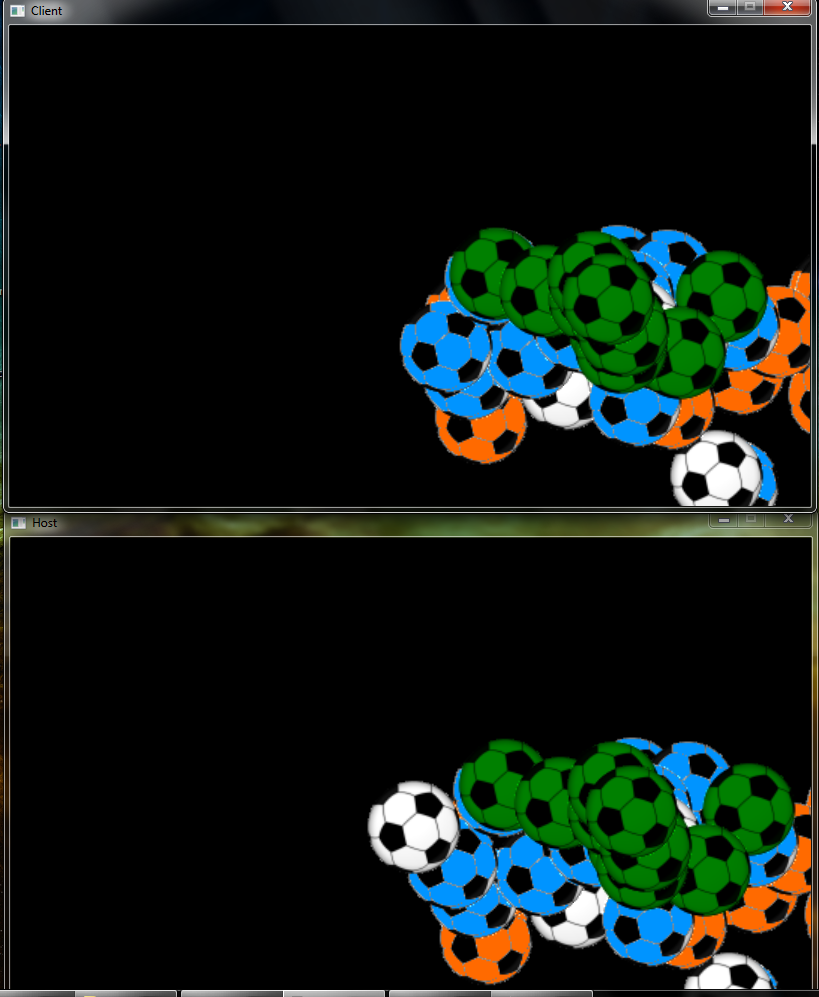
\includegraphics[width=8cm]{Pics/Networked_balls.png}
\end{center}
\caption{Networking sample}
\label{fig:networking_sample}
\end{figure}

The prototype is currently working. Figure \ref{fig:networking_sample} shows the bouncing balls sample in action, where we see that blue balls are generated by the client input, the red balls are generated by the host input, and the white balls are generated by the host script. % Figure [] shows the asteroid shooter sample where multiple ships cooperate in destroying falling asteroids.

%We have also studied some benchmarks on the two prototypes. The benchmarks show the bandwidth used by the samples with and without incremental transfers and local prediction, and they also show the average latency with and without lag compensation techniques.


\section{Future work}
Networking in Casanova is part of an appendix rather than the main work mainly because it is still incomplete. The implementation of the networking framework is still underway, and there is still not enough data to draw some conclusions and perform comparisons with other systems. Networking still requires an in-depth study of how to perform faster exploration of the game world with reflection (as discussed in Chapter \ref{chap:implementation}). Also, further optimizations such as updating some fields upon local update only, probabilistic updates from the host that take into account expected reliability of transmission to estimate which clients need what data, and a tracking server to move networked games on the Internet instead of limiting ourselves to local networks are being worked on.
